%%%%%%%%%%%%%%%%%%%%%%%%%%%%%%%%%%%%%%%%%
% This file was derived from:
% Journal Article
% LaTeX Template
% Version 1.4 (15/5/16)
%
% This template has been downloaded from:
% http://www.LaTeXTemplates.com
%
% Original author:
% Frits Wenneker (http://www.howtotex.com) with extensive modifications by
% Vel (vel@LaTeXTemplates.com)
%
% License:
% CC BY-NC-SA 3.0 (http://creativecommons.org/licenses/by-nc-sa/3.0/)
%
%%%%%%%%%%%%%%%%%%%%%%%%%%%%%%%%%%%%%%%%%

%----------------------------------------------------------------------------------------
%	PACKAGES AND OTHER DOCUMENT CONFIGURATIONS
%----------------------------------------------------------------------------------------

\documentclass[twoside,twocolumn]{article}

\usepackage{blindtext} % Package to generate dummy text throughout this template 

\usepackage[sc]{mathpazo} % Use the Palatino font
\usepackage[T1]{fontenc} % Use 8-bit encoding that has 256 glyphs
\linespread{1.05} % Line spacing - Palatino needs more space between lines
\usepackage{microtype} % Slightly tweak font spacing for aesthetics

\usepackage[english]{babel} % Language hyphenation and typographical rules

\usepackage[hmarginratio=1:1,top=32mm,columnsep=20pt]{geometry} % Document margins
\usepackage[hang, small,labelfont=bf,up,textfont=it,up]{caption} % Custom captions under/above floats in tables or figures
\usepackage{booktabs} % Horizontal rules in tables

\usepackage{lettrine} % The lettrine is the first enlarged letter at the beginning of the text

\usepackage{enumitem} % Customized lists
\setlist[itemize]{noitemsep} % Make itemize lists more compact

\usepackage{abstract} % Allows abstract customization
\renewcommand{\abstractnamefont}{\normalfont\bfseries} % Set the "Abstract" text to bold
\renewcommand{\abstracttextfont}{\normalfont\small\itshape} % Set the abstract itself to small italic text

\usepackage{titlesec} % Allows customization of titles
\renewcommand\thesection{\Roman{section}} % Roman numerals for the sections
\renewcommand\thesubsection{\roman{subsection}} % roman numerals for subsections
\titleformat{\section}[block]{\large\scshape\centering}{\thesection.}{1em}{} % Change the look of the section titles
\titleformat{\subsection}[block]{\large}{\thesubsection.}{1em}{} % Change the look of the section titles

\usepackage{fancyhdr} % Headers and footers
\pagestyle{fancy} % All pages have headers and footers
\fancyhead{} % Blank out the default header
\fancyfoot{} % Blank out the default footer
\fancyhead[C]{Running title $\bullet$ May 2016 $\bullet$ Vol. XXI, No. 1} % Custom header text
\fancyfoot[RO,LE]{\thepage} % Custom footer text

\usepackage{titling} % Customizing the title section

\usepackage{hyperref} % For hyperlinks in the PDF

% RMF additions
\usepackage{graphicx}
\usepackage{amsmath}
\interfootnotelinepenalty=1000 % default is 100; discourages splitting footnotes

%----------------------------------------------------------------------------------------
%	TITLE SECTION
%----------------------------------------------------------------------------------------

\setlength{\droptitle}{-4\baselineskip} % Move the title up

\pretitle{\begin{center}\Huge\bfseries} % Article title formatting
\posttitle{\end{center}} % Article title closing formatting
\title{Emergent Behavior in Graph Automata} % Article title
\author{%
\textsc{Richard Foard}\thanks{A thank you or further information} \\[1ex] % Your name
\normalsize Georgia Tech Research Institute \\ % Your institution
\normalsize \href{mailto:richard.foard@gtri.gatech.edu}{richard.foard@gtri.gatech.edu} % Your email address
}
\date{\today} % Leave empty to omit a date
\renewcommand{\maketitlehookd}{%
\begin{abstract}
\noindent A simple, rule-based
graph automaton was defined and simulated. Each of its possible rules specifies a set
of local topology and node state changes to be applied iteratively, starting with a random initial graph.
Simulation runs were performed using many different rules, each run terminating when its graph
collapsed or cycled.
Evolving and terminal graph states were analyzed macroscopically, using
aggregate statistics, and microscopically, by inspecting graph structures.
Results were compared with those from simulations of a machine that
iterated by applying random, rather than rule-based, changes. We found that...
\end{abstract}
}

%----------------------------------------------------------------------------------------

\begin{document}

% Print the title
\maketitle

%----------------------------------------------------------------------------------------
%	ARTICLE CONTENTS
%----------------------------------------------------------------------------------------

\section{Introduction}

\lettrine[nindent=0em,lines=3]{S} ince Alan Turing conceived his
universal machine in 1936, simple abstract automata have been studied. Interest broadened
beyond the theoretical realm in 1970,
when Conway published his \textit{Game of Life} simulations that highlighted the ability
of uncomplicated cellular automata to behave in complex ways. Researchers in the
nascent field of complexity theory also devoted attention to similar phenomena, such as the
"sandpile" first explored by Per Bak (true??).

In \textit{A New Kind of Science} (199?), Stephen Wolfram methodically analyzed
a variety of cellular automata types. His voluminous results cited particular inspiration from the
behavior of a one-dimensional machine running "Rule 110." Among his observations were... (list
irreducibility, etc.)

Wolfram and others have also suggested that some natural processes that were
previously thought to evolve by natural selection are instead
manifestations of things that nature found "easy" to accomplish using
the same fundamental principles that underlie simple automata.

In this work, we analyze a graph automaton -- a machine that operates on the same principles as
cellular automata, but runs using a graph rather than a "tape," or grid, as a substrate.
Where cellular machines define cell adjacency spatially, our machines use graph topology.

%------------------------------------------------

\section{Methods}

A rule-based automaton, \textbf{Machine C}, was designed and implemented in simulation.
The simulator was run repeatedly, using rules
selected at random from a large universe of possibilities. Measurements were recorded as the graphs
evolved through each run. The resulting database accumulated data on many thousands of runs. The body of data
was analyzed macroscopically, using aggregate
statistics, and microscopically, by inspecting statistical and graphic "snapshots" from individual runs.

Each simulation run begins with a randomly generated graph and progresses by
iteratively modifying its edges and node states; changes are made according to a rule selected
for the run. Each rule is effectively a simple program  that specifies, based on the state
of each node and its two topological neighbors, how local changes should be applied.

A simulation run proceeds as follows: (describe initial condition and iteration procedure)

\subsection{Graph Composition}

Nodes may be in one of two states: \textit{black} or \textit{white}.
Graph topology is narrowly restricted in order to simplify analysis:

\begin{itemize}
    \item Edges are directed.
    \item Nodes have out-degree of exactly two.
    \item Multiple, like-directed edges between two nodes are prohibited.
    \item "Self-linking" edges are permitted.
\end{itemize}

These conditions are established when creating initial graphs and maintained
throughout execution by "pruning" when necessary, as described in a later section.

An initial, random graph of size N is constructed by assigning two edges to each node, with
the destination of each selected at random from all nodes, observing the
constraint that both edges cannot have the same destination node. As a consequence,
all nodes have out-degree 2, but in-degree can vary from 0 to N. Each node is assigned
a \textit{black} or \textit{white} state at random, with equal likelihood.

\subsection{Machine \textbf{C} Rules and Operation}

At the start of each simulation run, a rule is selected and an initial graph
is generated.  The simulation proceeds in a series of
iterations. During each, the rule is applied at each node, yielding a draft
version of a new graph. The draft is then pruned to eliminate
prohibited structures, creating the input graph to the next iteration.

During an iteration, each node in the current graph is examined in turn.
Depending on the combined \textit{black}/\textit{white}
states of the node and its two neighbors, changes are made to the node's
state and its out-edges in the draft copy. Rules encode change
instructions as follows:

A rule consists of eight parts, each corresponding to a possible compound state of a node and its
two neighbors. Each rule-part specifies replacement values for
the node's state, the destination of its left out-edge, and the destination of its right
out-edge. A replacement node state is either \textit{black} or \textit{white}.
A replacement edge destination
(for purposes of description, it is convenient to designate a node's two out-edges "left" and "right.")
is one of:

\begin{itemize}
    \item L - the node's current left-edge destination
    \item R - the node's current right-edge destination
    \item LL - the current destination of its left neighbor's left-edge
    \item LR - the current destination of its left neighbor's right-edge
    \item RL - the current destination of its right neighbor's left-edge
    \item RR - the current destination of its right neighbor's right-edge
\end{itemize}
The process of a rule being applied to a node and its immediate neighbors is shown
schematically in (Fig. \ref{fig:Fig1}).

\begin{figure*}[tb] 
    \centering
    \makebox[\textwidth]{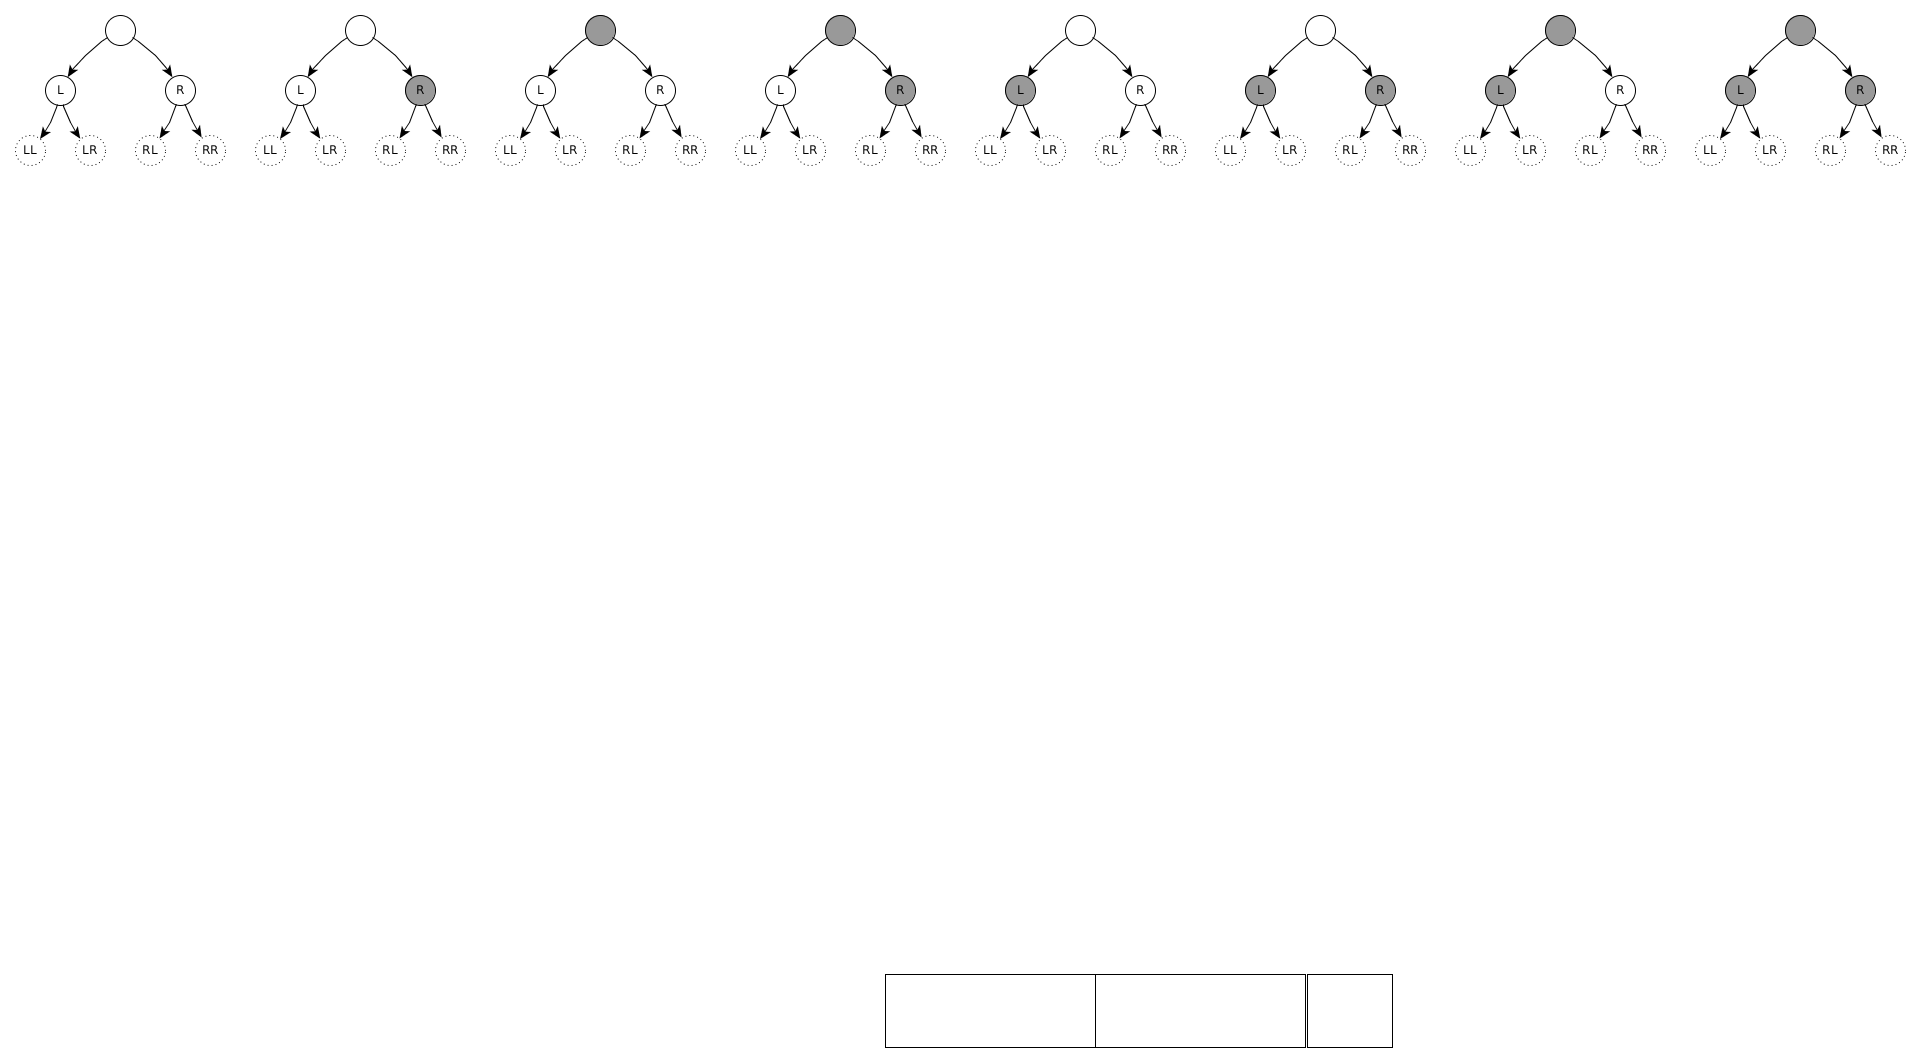
\includegraphics[width=.9\paperwidth]{./placeholder.png}}
    \caption{A rule specifies state-dependent changes to a node's state and its out-edges.}
    \label{fig:Fig1}
\end{figure*}

After all nodes in the original graph have been processed, pruning removes
any like-directed edges between pairs of nodes; pruning selectively removes nodes
and redirects edges, cascading as required until no prohibited structures remain.
If it is not empty, the pruned graph becomes the starting point for the next iteration;
if it is empty it is said to have collapsed.
The simulation run ends when (1) the graph collapses, (2) a state cycle is detected,
or (3) the maximum number of iterations is reached.

\subsection{Machine \textbf{C}'s Random Counterpart, \textbf{R}}

To gauge the extent to which machine \textbf{C} creates order out of
random starting graphs, a simulator for a second machine, \textbf{R},
was constructed. Like \textbf{C}, \textbf{R} makes iterative changes to the
graph, but proceeds by changing node states and edge assignments randomly
instead of under control of a rule. As with \textbf{C}, though, the scope
of \textbf{R}'s changes is limited to nodes' immediate topological neighborhoods.

\subsection{Pruning}

Invariants are maintained in all simulations.

\subsection{The Simulator}

Input parameters and statistics gathered. Data base and analysis tooling.
Constituent packages. How parameter values were selected and varied.

%------------------------------------------------

\section{Results}

Initial graphs are finite, rules are deterministic, and each iteration
either maintains the number of nodes or reduces it by pruning.
It is consequently certain that machine \textbf{C} will terminate for every rule,
either in a state cycle or in a graph collapse; it is likewise certain that
machine \textbf{R} will always terminate.
The possibility that a graph will traverse an astronomical number
of states\footnote{The number of possible states for an N-node graph is:
\[
2^N\cdot\binom{N}{2}^N
\]
}
before revisiting a previous configuration, however, limits the simulator's ability to
detect a cycle. For this reason, a third, "undetermined" category is included in
statistics on run outcomes.

Machine \textbf{C} is far less likely to produce graph collapses than
\textbf{R} is (59.3\% vs. 99.9\% of runs). In cases where \textbf{C} produces
collapses, average run length is consistently greater than
for \textbf{R} (Fig. \ref{fig:figA}). For both machine types, we refer to
the number of nodes at the end of the iteration immediately preceding a collapse,
or to the "settled" number of nodes in a cycling graph, as the terminal number of nodes.
(Add a note on the use of "neighbor" and separate into a separate paragraph on terms.)

\begin{figure}
  \fbox{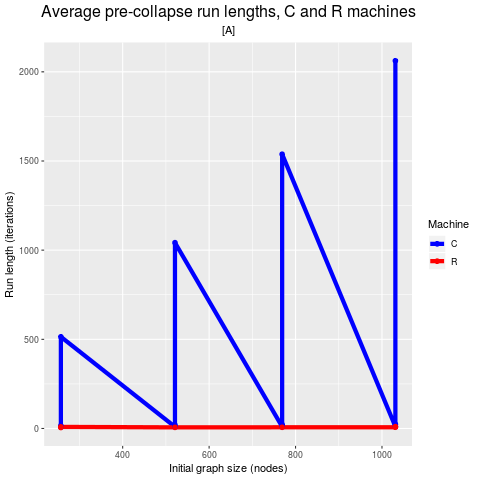
\includegraphics[width=\linewidth, scale=0.7]{figA.png}}
  \caption{On average, the rule-based \textbf{C} machine executes more iterations than \textbf{R} before collapse occurs.}
  \label{fig:figA}
\end{figure}

\subsection{Degree and Entropy}

Machine \textbf{C}, on average, generates graphs with a larger 
maximum in-degree than in the random case (Fig. \ref{fig:figC}), and also produces a
larger number of distinct in-degrees (Fig. \ref{fig:figB}).

\begin{figure}
  \fbox{\includegraphics[width=\linewidth, scale=0.7]{figC.png}}
  \caption{\textbf{C} produces a larger maximum in-degree than \textbf{R}.}
  \label{fig:figC}
\end{figure}

\begin{figure}
  \fbox{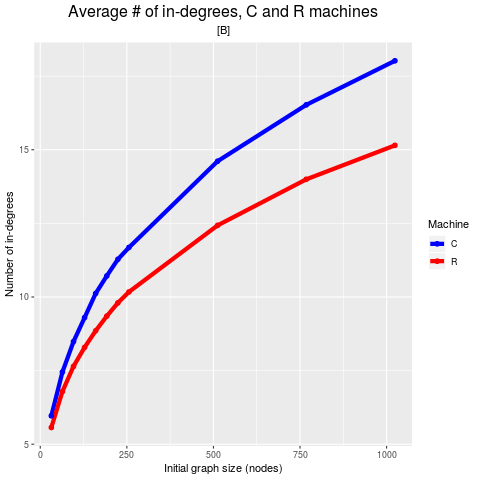
\includegraphics[width=\linewidth, scale=0.7]{figB.png}}
  \caption{\textbf{C} produces graphs with a larger number of in-degrees.}
  \label{fig:figB}
\end{figure}

Shannon's entropy [citation needed], computed on summary in-degree statistics and
normalized\footnote{Explanation of normalization}, can be regarded a measure of
a graph's "randomness."
As would be expected, entropy is consistently large in the randomly generated
initial graphs. Between the \textbf{R} and \textbf{C} machines, entropy in the terminal
graphs for \textbf{C} is lower than that for the randomly operating R (Fig. \ref{fig:figE}).
The drop in average entropy between initial graphs and the\textbf{R} machine's terminal
graphs seems surprising on its face, but is accounted for by the restriction that
\textbf{R}'s topological changes, like \textbf{C}'s, may only redirect a node's out-edge
to one of its own edges' destinations to one of its immediate neighbors'.
The effect is to "localize" the randomness, increasing apparent order in the graph.

\begin{figure}
  \fbox{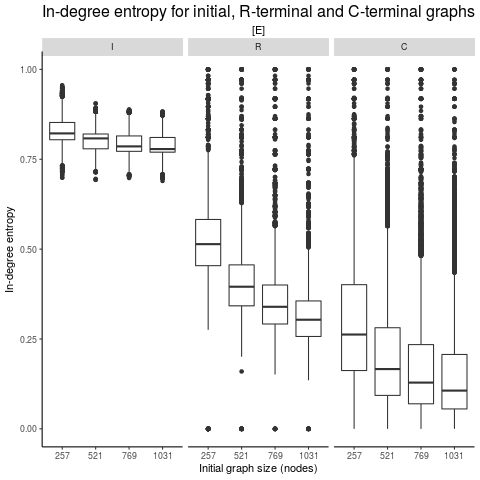
\includegraphics[width=\linewidth, scale=0.7]{figE.png}}
  \caption{In-degree entropy is largest in initial random graphs,
        smaller for \textbf{R}'s terminal graphs, and smallest for \textbf{C}'s terminal graphs.}
  \label{fig:figE}
\end{figure}

\subsection{Clustering}

Terminal clustering coefficients for machine \textbf{C} are smaller than those for \textbf{R} in
the large majority of cases (Fig. \ref{fig:figDd1024}).

\begin{figure}
  \fbox{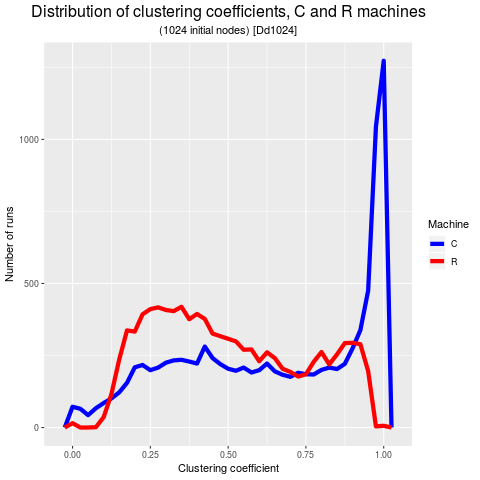
\includegraphics[width=\linewidth, scale=0.7]{figDd1024.png}}
  \caption{\textbf{C}'s average clustering coefficients are larger than \textbf{R}'s.}
  \label{fig:figDd1024}
\end{figure}

\subsection{Unhappy Endings -- Cycles and Collapses}

\subsection{Sensivity to Initial Conditions}

This is where things get more interesting.

For this one, we'll have to dust off the old self-organizing criticality
references. Are collapses like sandpile avalanches?

\subsection{Self-Organization -- Made to Order?}

\subsection{Learning the Hard Way}

\subsection{Analysis -- Doing the math}

\subsection{Evolution by Design}

\subsection{Interesting Configurations -- Photo Ops}

\subsection{In the Long Run...}

\begin{table}
\caption{Example table}
\centering
\begin{tabular}{llr}
\toprule
\multicolumn{2}{c}{Name} \\
\cmidrule(r){1-2}
First name & Last Name & Grade \\
\midrule
John & Doe & $7.5$ \\
Richard & Miles & $2$ \\
\bottomrule
\end{tabular}
\end{table}

Some dummy text was here.

\begin{equation}
\label{eq:emc}
e = mc^2
\end{equation}

Some dummy text was here.

%------------------------------------------------

\section{Discussion}

\subsection{Subsection One}

A statement requiring citation \cite{Figueredo:2009dg}.
Some dummy text was here, too.

\subsection{Subsection Two}

Some dummy text was here, too.

%----------------------------------------------------------------------------------------
%	REFERENCE LIST
%----------------------------------------------------------------------------------------

\begin{thebibliography}{99} % Bibliography - this is intentionally simple in this template

\bibitem[Figueredo and Wolf, 2009]{Figueredo:2009dg}
Figueredo, A.~J. and Wolf, P. S.~A. (2009).
\newblock Assortative pairing and life history strategy - a cross-cultural
  study.
\newblock {\em Human Nature}, 20:317--330.
 
\end{thebibliography}

%----------------------------------------------------------------------------------------

\end{document}
